\documentclass[a4paper,11pt]{article}
\input{/home/tof/Documents/Cozy/latex-include/preambule_lua.tex}
\newcommand{\showprof}{show them}  % comment this line if you don't want to see todo environment
\fancyhead[L]{Stéganographie}
\newdate{madate}{10}{09}{2020}
%\fancyhead[R]{\displaydate{madate}} %\today
\fancyhead[R]{Seconde - SNT}
%\fancyhead[R]{Première - NSI}
%\fancyhead[R]{Terminale - NSI}
\fancyfoot[L]{~\\Christophe Viroulaud}
\AtEndDocument{\label{lastpage}}
\fancyfoot[C]{\textbf{Page \thepage/\pageref{lastpage}}}
\fancyfoot[R]{\includegraphics[width=2cm,align=t]{/home/tof/Documents/Cozy/latex-include/cc.png}}
\usepackage{tikz}

\begin{document}
\begin{Form}
\begin{commentprof}
mettre \textbf{steganographie.zip} sur site
\end{commentprof}
\section{Problématique}
La stéganographie est l'art de la dissimulation. Le principe est de cacher un message dans un autre message. Il est ainsi possible de cacher une image dans une autre image.
\begin{center}
\shadowbox{\parbox{16cm}{\centering Comment les informations d'une image sont-elles codées dans la mémoire de l'ordinateur?}}
\end{center}
\section{Notation binaire}
\begin{aretenir}[]
Un \textbf{bit} est la plus petite unité de stockage. Il ne peut contenir qu'une valeur parmi 0 ou 1.
\end{aretenir}
Pour stocker une couleur on a besoin de huit bits (\textbf{1 octet}).
\begin{center}
\begin{tabular}{|c|c|}
\hline 
couleurs & bits \\ 
\hline 
0 & 00000000 \\ 
\hline 
1 & 00000001 \\ 
\hline 
2 & 00000010 \\ 
\hline 
... & ... \\ 
\hline 
239 & 11101111 \\ 
\hline 
240 & 11110000 \\ 
\hline 
... & ... \\ 
\hline 
254 & 11111110 \\ 
\hline
255 & 11111111 \\ 
\hline 
\end{tabular} 
\end{center} 
On peut différencier les huit bits en deux catégories:
$$\underbrace{\text{\Huge{1 1 1 1}}}_{\text{bit de poids fort}}~\underbrace{\text{\Huge{1 1 1 1}}}_{\text{bit de poids faible}}$$
\begin{activite}
\begin{enumerate}
\item Se rendre sur le site \url{https://htmlcolorcodes.com/fr/} .
\item Choisir la couleur rouge (R = 255, G = 0, B = 0).
\item La comparer avec le rouge (R = 240, G = 0, B = 0).
\item Que peut-on dire des rouges compris entre 240 et 255?
\item Comparer l'écriture binaire de ces couleurs.
\end{enumerate}
\end{activite}
\section{Principe de la stéganographie}
En ne gardant que les bits de poids fort pour chaque couleur, l'image n'est que très peu dégradée. Le principe de la dissimulation est de placer les bits de poids fort de l'image secrète à la place des bits de poids faible de l'image visible.
\begin{center}
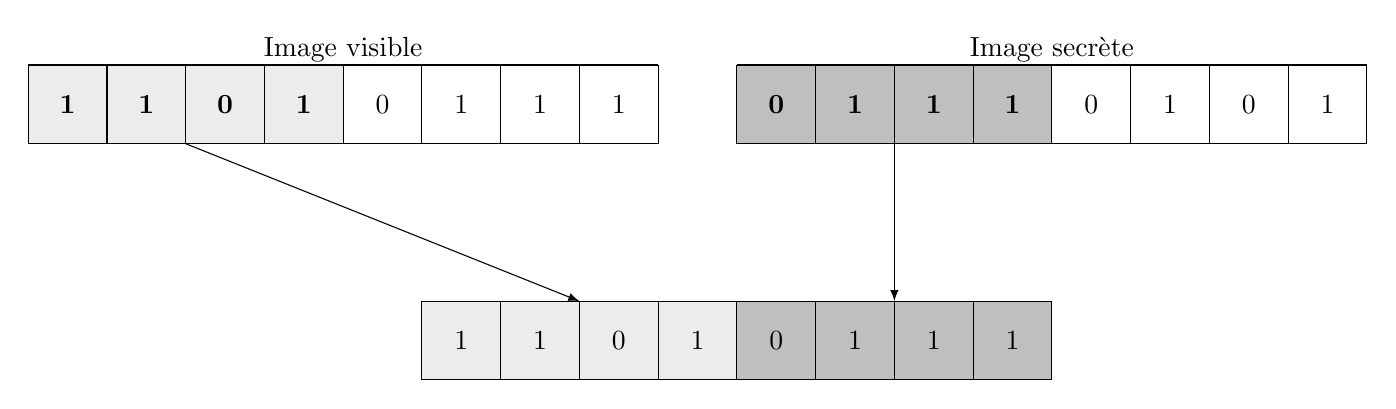
\begin{tikzpicture}
\node (im1) at (4,1.2) {Image visible};
\fill [gray!15] (0,0) rectangle (4,1);
\draw (0,0) grid (8,1);
\node (0) at (0.5,0.5) {\textbf{1}};
\node (1) at (1.5,0.5) {\textbf{1}};
\node (2) at (2.5,0.5) {\textbf{0}};
\node (3) at (3.5,0.5) {\textbf{1}};
\node (4) at (4.5,0.5) {0};
\node (5) at (5.5,0.5) {1};
\node (6) at (6.5,0.5) {1}; 
\node (7) at (7.5,0.5) {1}; 

\node (im2) at (13,1.2) {Image secrète};
\fill [gray!50] (9,0) rectangle (13,1);
\draw (9,0) grid (17,1);
\node (10) at (9.5,0.5) {\textbf{0}};
\node (11) at (10.5,0.5) {\textbf{1}};
\node (12) at (11.5,0.5) {\textbf{1}};
\node (13) at (12.5,0.5) {\textbf{1}};
\node (14) at (13.5,0.5) {0};
\node (15) at (14.5,0.5) {1};
\node (16) at (15.5,0.5) {0}; 
\node (17) at (16.5,0.5) {1}; 

\fill [gray!15] (5,-3) rectangle (9,-2);
\fill [gray!50] (9,-3) rectangle (13,-2);
\draw (5,-3) grid (13,-2);
\node (20) at (5.5,-2.5) {1};
\node (21) at (6.5,-2.5) {1};
\node (22) at (7.5,-2.5) {0};
\node (23) at (8.5,-2.5) {1};
\node (24) at (9.5,-2.5) {0};
\node (25) at (10.5,-2.5) {1};
\node (26) at (11.5,-2.5) {1}; 
\node (27) at (12.5,-2.5) {1}; 

\draw[->,>=latex] (2,0) to (7,-2);
\draw[->,>=latex] (11,0) to (11,-2);
\end{tikzpicture}
\captionof{figure}{Cacher une image dans une autre.}
\label{stegano}
\end{center}
\begin{activite}
\begin{enumerate}
\item Détailler les étapes du protocole pour cacher une image secrète dans une image visible.
\item Télécharger le fichier \emph{steganographie.zip} sur le site \url{https://cviroulaud.github.io}  et extraire les dossiers.
\item Ouvrir le logiciel \emph{Spyder}.
\item Dans le dossier \emph{cacher} ouvrir le programme \emph{cacher-image.py} .
\item Observer le code. Quelles lignes permettent de sélectionner les bits de poids fort de l'image secrète?
\item Compléter les lignes 11 et 12 pour cacher l'image de l'éléphant dans l'image du magasin de porcelaine.
\item Observer l'image obtenue. L'éléphant est-il correctement caché?
\end{enumerate} 
\end{activite}
\section{Retrouver une image cachée}
Un fabricant de smartphone vous a envoyé la photographie du prototype de son nouvel appareil. Afin de rester discret l'image est cachée dans une autre.
\begin{activite}
\begin{enumerate}
\item Dans le dossier \emph{retrouver} ouvrir l'image mystère. Peut-on distinguer l'image cachée?
\item Avec \emph{Spyder} ouvrir le programme \emph{retrouver-image.py} .
\item Compléter la ligne 11.
\item Quel est le rôle des lignes 20 à 22?
\item Exécuter le programme pour retrouver l'image cachée.
\end{enumerate}
\end{activite}
\end{Form}
\end{document}